% Updated in February 2016 by Hwann-Tzong Chen
% Updated in May 2014 by Hideo Saito
% Updated in March 2012 by Yasuyuki Matsushita
% Updated in April 2002 by Antje Endemann, ...., and in March 2010 by Reinhard Klette
% Based on CVPR 07 and LNCS style, with modifications by DAF, AZ and elle 2008, AA 2010, ACCV 2010

\documentclass[runningheads]{llncs}
\usepackage{graphicx}
\usepackage{amsmath,amssymb} % define this before the line numbering.
\usepackage{ruler}
\usepackage{color}
\usepackage{subfigure}
\usepackage{mathrsfs}
%===========================================================
\begin{document}
\pagestyle{headings}
\mainmatter

\def\ACCV16SubNumber{***}  % Insert your submission number here

%===========================================================
\title{Building Rooftop Extraction in Aerial Image with Dual-Task Fully Convolutional Network} % Replace with your title
\titlerunning{ACCV-16 submission ID \ACCV16SubNumber}
\authorrunning{ACCV-16 submission ID \ACCV16SubNumber}

\author{Anonymous ACCV 2016 submission}
\institute{Paper ID \ACCV16SubNumber}

\maketitle
%===========================================================
\begin{abstract}
   Automatic building extraction from remote sensing image plays a critical role in  a diverse range of applications. However, it is  a huge challenge to recognize buildings accurately and extract their contours precisely in a complex natural environment at the same time. To address this problem, we present a dual-supervision fully convolutional network(DSFCN) for building extraction. One task is detecting buildings with different sizes in aerial image, 
an advanced multi-scale fusion strategy is introduced. The other task is delineating a clearer boundary of buildings, we propose a new training technique which more focuses on neighbourhood of edge. The experiment results test on a publicly available aerial imagery dataset proved that our proposed  methodology significantly  shorten  time-consuming and surpass the performance of state-of-the-art.

\end{abstract}

%===========================================================
\section{Introduction}
   With the rapid development of remote sensing technologies and popularization of geospatial related commercial software, very high resolution satellite images are very easily accessible, these valuable data provides a huge fuel for interpreting real terrestrial scenes. Building rooftops is one the most important part of terrestrial objects because it is essential for a wide range of technologies, such as, urban planning, automated map making, 3D city modelling, disaster assessment, military reconnaissance, etc. However, it is  very costly and time-consuming for human experts to complete this task. Therefore, many researchers have made massive attempts to extract buildings automatically. 

% Though a series of approaches have been proposed to solve this problem, it is still a big challenge to  
%build a genetic and robust building extraction system. This is mainly due to the following two reasons. One is that a large amount of buildings are occluded by shadows stem from itself or other buildings, it causes a significant difficulty for image segmentation. The other is that building rooftops possess diverse shapes and colors, therefore, they can be easily confused with similar objects such as cars, roads, and courtyards. 

   In previous literatures, large amounts of efforts achieve good performance in extracting buildings with special color, shapes, textures, or surroundings. According to the information they concerned, these methods may fall into three classes. Though these techniques are different, the common character of them is there are a series of manually set rules or features in their system.
   
   One popular way of extracting buildings is employing their shape information. It is observed that rooftops have more regular shapes, which usually are rectangular or combinations of several rectangles. A dozen years ago, Noronha and Nevatia \cite{noronha2001detection} designed a system that detects and constructs 3D models for rectilinear buildings from multiple aerial images. Firstly, hypotheses for rectangular rooftop were generated by grouping lines, then they were verified by searching for presence of predicted walls and shadows. Nosrati and Saeedi \cite{nosrati2009novel} pointed out that polygonal rooftops correspond to closed loops in a graph which represents the relationship between intersections of a pair of edge in an efficient way. In \cite{izadi2012three}, Izadi and Saeedi exploited a graph-based search to establish a set of rooftop hypotheses through examining the relationships of lines and line intersections. Cui \textit{et al.} \cite{cui2012complex} extracted buildings through the Hough transform (HT), but HT has notable drawbacks in parameter tuning and time complexity. Cote and Saeedi \cite{cote2013automatic} generated rooftop outline from selected corners in  multiple color and color-invariance spaces, further refined to fit the best possible boundaries through level-set curve evolution. In \cite{wang2015efficient}, Wang \textit{et al.}  presented a graph search-based perceptual grouping approach to hierarchically group line segments detected by EDLines \cite{akinlar2011edlines} into candidate rectangular buildings, computation complexity of the approach was reduced dramatically compared to \cite{noronha2001detection} \cite{izadi2012three} \cite{cote2013automatic} \cite{mayunga2007semi}. However, geometric primitives based methods suffer from three serious shortcomings. Firstly, they lack the ability of detecting arbitrarily shaped building rooftop. Secondly, they fail to  extract credible geometric features in buildings with inhomogeneous color distribution or low contrast with surroundings. Thirdly, it is hardly possible to process large-scale scenes because of their high computational-complexity.	
	
	Several studies reported that buildings are often composed of homogeneous regions with similar color or texture nearby shadows in remote sensing images. Spectral features is a distinctive feature for object detection, for instance, shadows are commonly dark grey or black, vegetations are usually green or yellow with particular textures, and main roads are dim gray with different road marks in most case. According to these prior knowledge mentioned above, Ghaffarian \textit{et al.}  \cite{ghaffarian2014automaticPFICA} proposed an purposive fast independent component analysis (PFastICA) technique to separate building area from remote sensing image. However, Ghaffarian's approach fails to detect the buildings with significantly different coloured rooftops. In \cite{ghaffarian2014automaticsupervised}, illumination direction and shadow area information of training samples were collected firstly, and then a improved parallelepiped classification method was applied to classify the image pixels into building and non-building areas. In \cite{chen2014shadow}, Chen \textit{et al.} proposed a supervised building detection framework. At first, source image was divided into super-pixels using the SLIC \cite{achanta2012slic} algorithm, then shadow patches are recognized using LDA color feature and the SVM classifier. The rough segmentation of buildings is employed by an adaptive regional growth algorithm that considers the spatial relationship between shadows and buildings. Finally, buildings are segmented accurately using a level set model. Dornaika \textit{et al.} \cite{dornaika2015object} proposed a similar framework,
Firstly, remote sensing image is segmentation  by statistical region merging (SRM) algorithm , hybrid descriptor composed by color histograms and local binary patterns is used to represent each segmented region. Finally, each region was classified using machine learning tools and a gallery of training descriptors. However, a major problem of these methods is that they have less capability to detect building rooftop with significantly varying illumination in different parts or no surrounding shadows.

   Other studies presented synthetic approaches with fusion of multiple features to extract building footprints from aerial images. Baluyan \textit{et al.} \cite{baluyan2013novel} proposed a method combining spectral and spatial features. Firstly, image is segmented into a set of rooftop candidates. Secondly, a SVM classifier is trained to distinguish rooftop regions or nonrooftop regions using extracted multiple features in dataset. Finally, "histogram method" is devised to detect missed rooftops in previous step. In \cite{ngoautomatic}, Ngo \textit{et al.} presented a novel approach for automated detection of rectangular buildings. At the first step, image is decomposed into small homogeneous regions as candidates. At the second step, a merging process is then performed over regions having similar spectral traits to produce rectilinear building region in accordance with position of shadows. Li \textit{et al.} \cite{li2015robust} proposed a higher order conditional random field (HCRF) based method, which incorporates both pixel-and segment-level information for the segmentation of rooftops. They claimed that the proposed model outperforms the best unsupervised methods at rooftops with complex structures and sizes. Nonetheless, feature selection and parameter tuning are considerable troubles.
    
   In recent years, deep neural networks have been widely deployed in general image segmentation or scene labelling tasks. Mnih \cite{Mnih2013Machine} presented a patch-based framework for learning to label aerial images. A carefully designed neural network architecture is designed for predicting buildings in aerial imagery, and then the output of this network is processed by conditional random fields(CRFs). Satito \cite{Saito2016Multiple} improved Mnih's networks for extracting multiple kinds of objects simultaneously, two techniques consisting of model averaging with spatial displacement(MA) and channel-wise inhibited softmax (CIS) are introduced to enhance the  performance. 
However, these two methods need to crop test image into a standard size, which not only  increase the time loss, but also break the integrity of building. In many applications, especially in city modelling, precise building boundary is a matter of considerable interest.  Therefore, it is necessary to develop a system that possesses high recognition accuracy and  boundary precision.
   
  In this article, we propose a dual-supervision fully convolutional network(DSFCN), as the name suggests, which complete two tasks only in a single convolutional neural network. Long and Shelhamer \cite{Long2014Fully} firstly propose the concept of fully convolutional network(FCN), which turns out to be  appropriate to complete semantic segmentation task. FCN takes whole image as inputs and directly outputs building rooftops by one pass of forward propagation. Because it can process input images of any sizes without warping or cropping, integrality of object is protected much better. However, it has less ability to  process a large number of small buildings in aerial image.  For the sake of handling this problem, we integrate all predictions from convolutional layers with skipped receptive fields. Moreover, a new loss functions is designed to train whole network for  labelling buildings accurately and keeping footprint of  buildings precisely. As far as we know, it is the first case to consider these two tasks in building extraction in a sole network.
  
  The rest of this article is organized as follows. The section 2.1 outlines some key ideas of fully convolutional network(FCN), the section 2.2 provides a brief overview of our neural network architecture. In section 3, two kinds of new loss functions is proposed. The section 4.1  presents the datasets which is used for training and testing in our experiments. The section 4.2  introduces training settings and strategies of our proposed network.  The section 4.3  compares  performances using different loss functions mentioned in section 3 by two well-know metrics. In section 4.4, we compare our results with two best methods using same dataset with us. In section 5, we discuss the experimental results and summarize whole article.
	
%===========================================================
\section{Network Architecture}
     In this section, we firstly introduce a well-know semantic segmentation network, called fully convolutional network(FCN)\cite{Long2014Fully}. We attempt to extract footprints of building  using  architecture proposed by author and two modified versions. Our experiments show that these networks are not enough to accomplish building   extraction task. \textbf{Therefore, we introduce a multi-scale network for extracting rooftops, it turns out to be achieve state-of-the-art performance in a public aerial image dataset. }
     
\subsection{Fully Convolutional Network}
	Based on the observation of our dataset, we learned that buildings have various sizes and shapes. So, it is not reasonable to employ image patches which are cropped into a fixed size as the neural network input. As for as we know, fully convolutional network(FCN) takes whole image as inputs and directly outputs building rooftops by one pass of forward propagation. Because it can process input images of any sizes without warping or cropping, integrality of object is protected much better.
	
	 Long  \textit{et al.} put forward the concept of fully convolutional network(FCN) in \cite{Long2014Fully} for the first time. \textbf{It said: "While a general deep net computes a general nonlinear function, a net with only layers of this form computes a nonlinear filter, which we call a deep filter or fully convolutional network".} In practice, the fully connected layers in traditional CNNs are transformed to convolutional layers with 1 $\times$ 1 kernels. Due to the mechanism of pooling, the output of the network is a coarse heat map. For pixelwise prediction, skip-net technique is used to connect various coarse outputs back to pixels.  For example, the framework of FCN-8s (see Fig. \ref{fig:Fig1FCN8s}) is described as following. We firstly obtain the 16 stride predictions by fusing the predictions of pooling4 with the 2 $\times$ upsampling of predictions from \textit{conv7}(convolutionalized \textit{fc7}). Then we continue in this fashion by fusing predictions from \textit{pool3} with a 2 $\times$ upsampling of the 16 stride predictions, denoted as 8 stride predictions. Finally, the 8 stride predictions are upsampled back to image with original size. 
	 
	 In our experiments, we first directly apply the FCN-8s to extract building rooftop by replacing the loss function with sigmoid cross-entropy loss. In order to achieving better performance, the network is extended to FCN-4s, FCN-2s. Our experiments show that FCN-4s and FCN-2s get the best performance with overall recall of 70.19 $\%$ in break-even point. According to our results, the first row of Fig. \ref{fig:FCN4s-results} indicate that FCN-4s has less ability to handle  objects with small size. The second row of Fig. \ref{fig:FCN4s-results} shows that it is hard for FCN to discriminate buildings with ground if their color is similar. To overcome these drawbacks, a improved FCN is introduced in next section.
	 
\begin{figure}
\centering
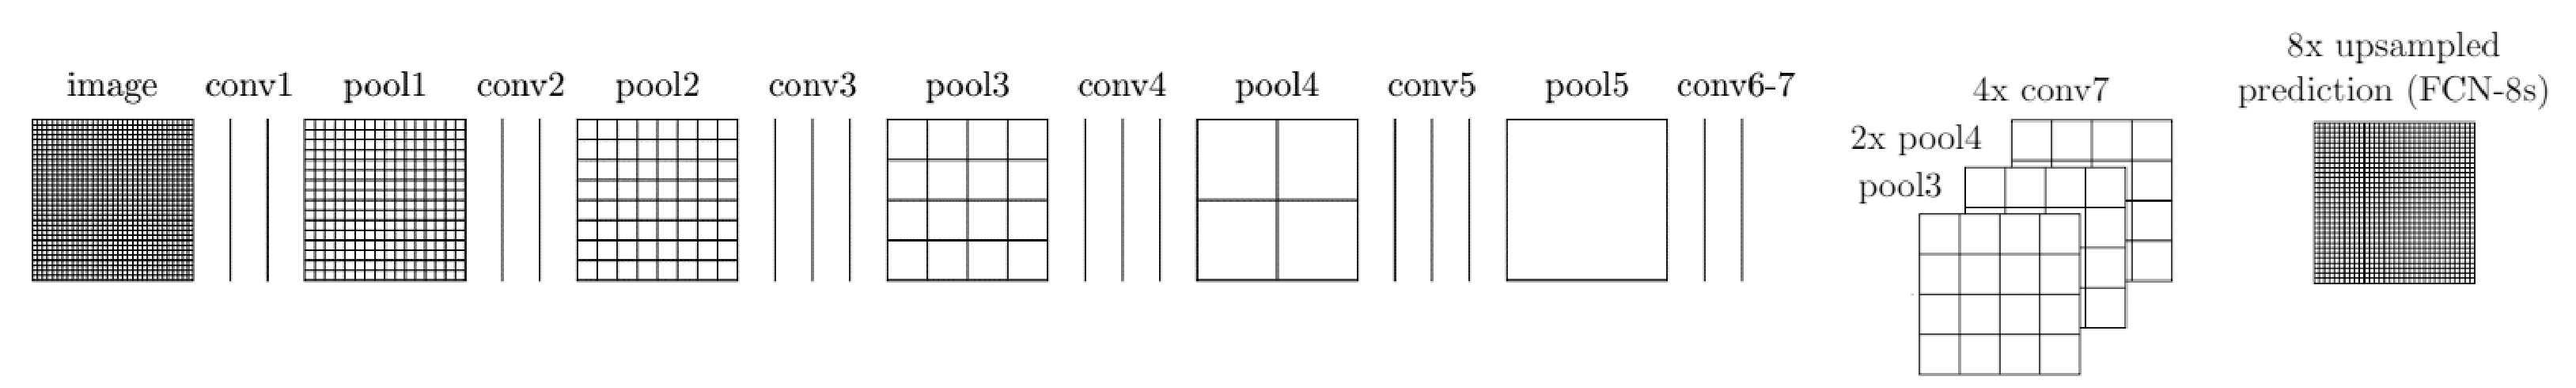
\includegraphics[width=120mm]{FCN8s}
\caption{The framework of FCN-8s}
\label{fig:Fig1FCN8s}
\end{figure}
	
\begin{figure}
\centering
\subfigure[]{	
	\label{fig:InputImage}
	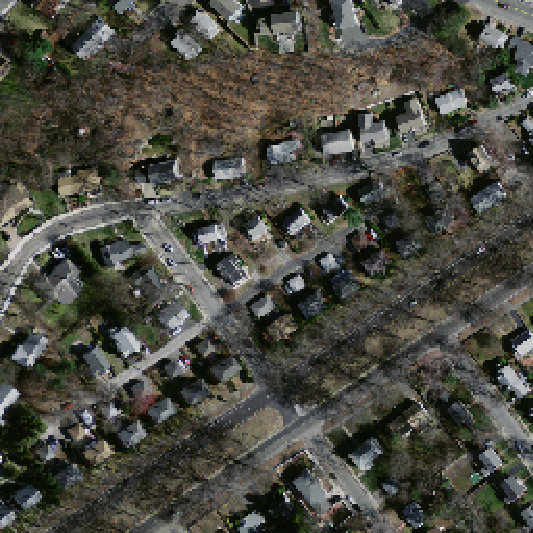
\includegraphics[width=35mm]{FCN4s-results-Input(a)}}
\subfigure[]{
	\label{fig:GroundTruth}
	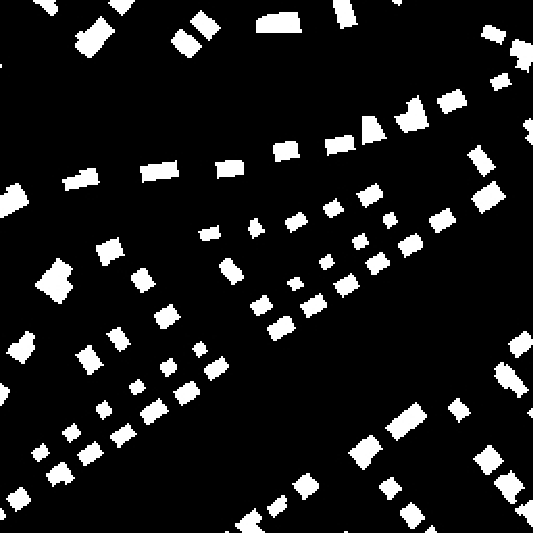
\includegraphics[width=35mm]{FCN4s-results-GT(b)}}
\subfigure[]{
	\label{fig:FCN-4s}
	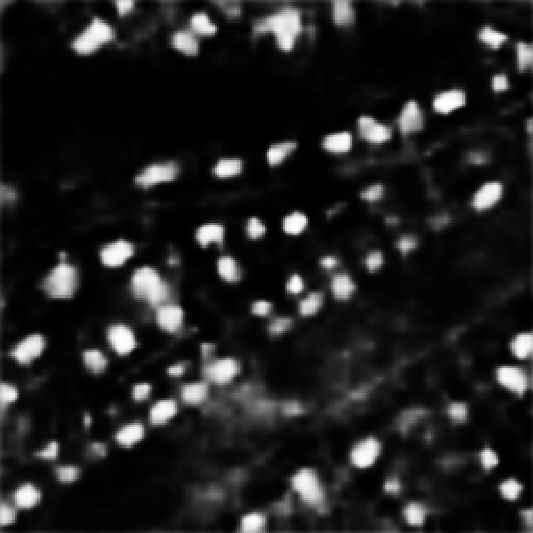
\includegraphics[width=35mm]{FCN4s-results-Prediction(c)}}
\subfigure[]{	
	\label{fig:InputImage}
	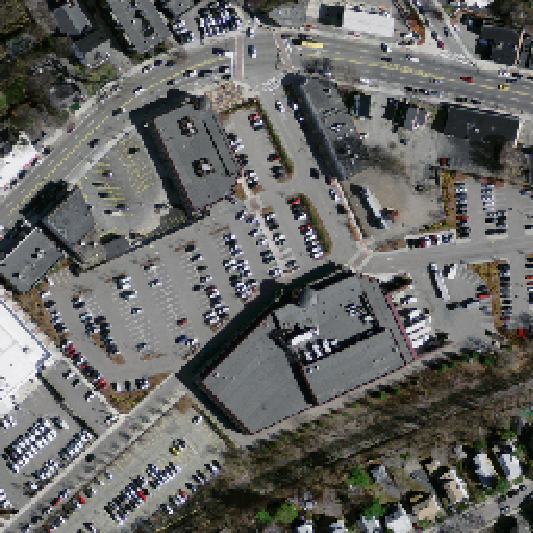
\includegraphics[width=35mm]{FCN4s-results-Input(d)}}
\subfigure[]{
	\label{fig:GroundTruth}
	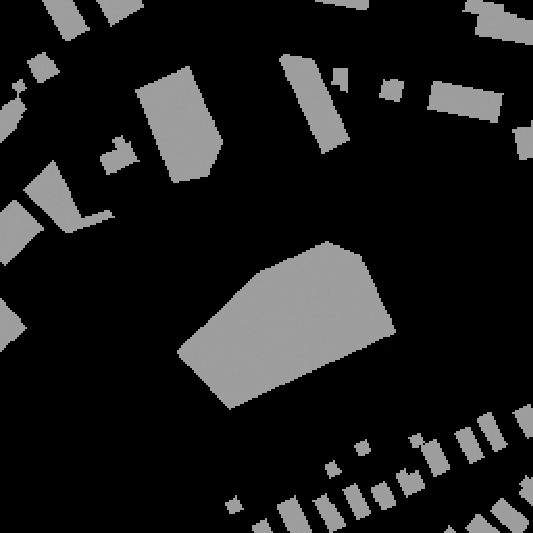
\includegraphics[width=35mm]{FCN4s-results-GT(e)}}
\subfigure[]{
	\label{fig:FCN-4s}
	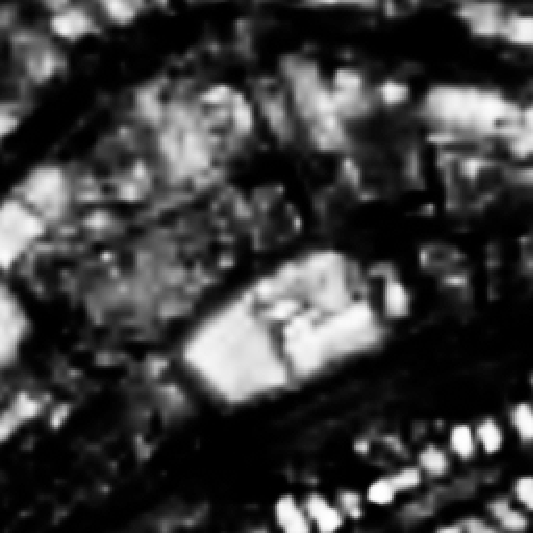
\includegraphics[width=35mm]{FCN4s-results-Prediction(f)}}
\caption{(a),(d) Input image. (b),(e) Ground truth. (c),(f) FCN-4s prediction.}
\label{FCN4s-results}
\end{figure}
 
\subsection{Our Architecture}  
    There are two main  
   (1) Last stage of VGGNet is cut, including the 5th pooling layer and all the fully connected layers. Because a layer with stride 32 yields a too-small output plane with the consequence that the interpolated prediction map will be too fuzzy to utilize. (2) In order to integrating multi-scale predictions, we connect some output layers to the last convolutional layer in each stage, respectively conv1$\_$2, conv2$\_$2, conv3$\_$3, conv4$\_$3, conv5$\_$3. Xie and Tu \cite{Xie2015Holistically} have proved this network archive good performance for edge detection. Edge detection work on a very fine level, and our system need to extract many tiny objects, so, it is reasonable to utilize the similar architecture to extract rooftops.
 	
\begin{figure}
\centering
\includegraphics[width=90mm]{ourArchitecture}
\caption{Our Network Architecture}
\label{fig:ourArchitecture}
\end{figure}1

\section{Proposed Method}
    Our goal is to predict probabilistic label image $\mathbf{M}$ from an input aerial image $\mathbf{S}$. Fig \ref{fig:ResultsofDifferentSupervision} shows an example of $\mathbf{S}$ and $\mathbf{M}$. We directly learn a mapping from raw pixels in $\mathbf{S}$ to a true label image  $\mathbf{M}$ by training the whole network. In this section, we give the mathematical definition of the problem, and a standard loss function is introduced using our formulation thereafter. In practice, building boundaries play a more important role than its inner parts, thus, we give more attention to pixels around building's contour. A new loss function is defined to handle this problem, the experiment results is shown in \ref{fig:DoubleLoss}.
    
\subsection{Formulation}
    Here we formulate our approach for building extraction. We denote our input training data set by $\mathbf{I} = \{(\mathbf{S}_{n},\mathbf{M}_{n}),n = 1,\ldots,\vert \mathbf{S}_n \vert \}$, where sample $\mathbf{S}_{n} = \{s_{j}^{(n)}, j = 1,\ldots,\vert \mathbf{S}_n \vert \}$ denotes the raw input image and  $\mathbf{M}_{n} = \{m_{j}^{(n)}, j = 1,\ldots,\vert \mathbf{S_n} \vert\}$, $m_j^{(n)} \in \{0,1\}$ denotes the corresponding ground truth binary labelling map for satellite image $\mathbf{S}_{n}$.  Taking account of each image holistically and independently, thus, we adopt the subscript $n$ for notational simplicity. Our goal is to have a network that learns features from which it is possible to produce building maps approaching the ground truth. 
    In our image-to-image training, the loss function is computed over all pixels in a training image $\mathbf{S} = \{s_{j}, j = 1,\ldots,\vert \mathbf{S} \vert\}$ and building map $\mathbf{M} = \{m_{j}, j = 1,\ldots,\vert \mathbf{S} \vert\}$, $m_j \in \{0,1\}$.
For simplicity, we denote the collection of all standard network layer parameters as $\mathbf{W}$. For each pixel $j$ in a training image, the possibility that assigns it to building is denoted as $\hat{m}_j = Pr(m_j = 1|\mathbf{S};\mathbf{W})$. Specifically, the definition of sigmoid cross-entropy loss function is shown in Eq (\ref{single-loss}).
\begin{equation}
	\label{single-loss}
    \mathcal{L}_{single} = - \sum_{j \in \mathbf{S}} \left[ m_j \log{\hat{m}_j} + (1 - m_j)\log{(1 - \hat{m}_j)} \right]
\end{equation}

\subsection{Structure-focused Learning}
    In order to obtain precisely structure, we define a weighted loss function which gives more attention to building's boundary. It is desirable to have a representation that encodes all boundaries as well as region masks. The signed distance function  is quite appropriate choice. The signed distance function value at a pixel is equal to the distance from the pixel to its closest point on boundaries with positive indicates inner of objects and negative otherwise. Fig. \ref{fig:OutRepresentation}. In our system, we define marginal area $\mathbf{E}$ as all pixels those absolute value of value in distance map are less than a certain threshold. In marginal area, we increase the loss weight according to its value in distance map. We assume that influence of miss labelled pixels which far from boundary is relatively larger than near ones. That is to say, we expect that the predicted contour is fitted to ground truth as good as possible. To achieve this goal, we modify the standard   sigmoid cross-entropy loss by adding a bound term. The equation is shown in Eq. \ref{double-loss}.  
       
 \begin{equation}
	\label{double-loss}
	\begin{aligned}
	 \mathcal{L} = - \sum_{j \in \mathbf{S}} \left[ 1\{m_j >= 0\} \log{\hat{m}_j} + 1\{m_j < 0\}\log{(1 - \hat{m}_j)} \right] \\
     - \beta \sum_{j \in \mathbf{E}} e^{\alpha \vert d_j \vert}  \left[ 1\{m_j >= 0\} \log{\hat{m}_j} + 1\{m_j < 0\} \log{(1 - \hat{m}_j)} \right]
	\end{aligned}
 \end{equation}
 
% \begin{figure}
% \label{OutRepresentation}
% \centering
% \subfigure[Aerial image]{	
%	\label{fig:AerialImage}
%	\includegraphics[width=30mm]{OutRepresentation(AerialImage)}}
% \subfigure[Region Mask]{
%	\label{fig:LabellingMap}
%	\includegraphics[width=30mm]{OutRepresentation(LabellingMap)}}
% \subfigure[Signed Distance Map ]{
%	\label{fig:SingleLoss}
%	\includegraphics[width=30mm]{OutRepresentation(SignedDistanceMap)}}
% \caption{Two output representations}
% \end{figure}
%===========================================================
\section{Experiments}
In this section, we discuss our detailed implementation and report the performance of our proposed algorithm.

\subsection{Dataset}
In our experiments, we use \textit{Massachusetts Buildings Dataset} (Mass. Buildings) proposed by Mnih \cite{Mnih2013Machine} and publicly available on website
http://www.cs.toronto.e
du/~vmnih/data/. The dataset consists of 151 aerial images of the Boston area, with each of the images being 1500 $\times$ 1500 pixels for an area of 2.25 square
kilometers. Hence, the entire dataset covers roughly 340 square kilometers. The data is split into a training set of 137 images, a test set of 10 images and
a validation set of 4 images. To train the network, we create image tiles of size 256 $\times$ 256 by means of cropping entire image using a sliding window with size of 256 $\times$ 256 and stride of 64 pixels. When scanning the whole dataset, image tiles with too many white pixels are removed. After scanning, train and validation dataset consists of 75938 and 2500 tiles and corresponding building masks. For testing, we use ten 1500 $\times$ 1500 entire images covering area excluded from the training data. 
In our experiments, input image should be scaled into range [0,1]. 

\subsection{Implementation}
The implementation of our framework is based on the publicly  available \textit{Caffe} \cite{Jia2014Caffe} Library. In our system, the whole network is fine-tuned from an initialization with the pre-trained VGG-16 Net model. Thus, it cost about four hour for training the network after 4000 iterations on a single NVIDIA Titan 12GB GPU.

The network is trained in an end-to-end manner. No pre or post-processing is used. We train the networking using stochastic gradient descent with 20 images as a mini-batch. The weight update rule is used with fixed learning rate $10^{-5}$, momentum 0.9, and weight decay $5\times 10^{-3}$. To prevent gradient decreasing significantly, clip$\_$gradients is set to 10000. 

\subsection{Results}
 
%\begin{figure}
%\centering
%\subfigure[Aerial image $\mathbf{S}$]{	
%	\label{fig:AerialImage}
%	\includegraphics[width=30mm]{Fig4(a)}}
%\subfigure[Labelling map $\mathbf{M}$]{
%	\label{fig:LabellingMap}
%	\includegraphics[width=30mm]{Fig4(b)}}
%\subfigure[Single supervision predicted result $\hat{\mathbf{M}}_{single}$ ]{
%	\label{fig:SingleLoss}
%	\includegraphics[width=30mm]{Fig4(c)}}
%\subfigure[Double supervision predicted result $\hat{\mathbf{M}}_{double}$ ]{
%	\label{fig:DoubleLoss}
%	\includegraphics[width=30mm]{Fig4(d )}}
%\caption{Compared results of using different supervisions}
%\label{ResultsofDifferentSupervision}
%\end{figure}

%===========================================================
\section{Conclusions}


%===========================================================
\bibliographystyle{splncs}
\bibliography{egbib}

%this would normally be the end of your paper, but you may also have an appendix
%within the given limit of number of pages
\end{document}
